\documentclass[aspectratio=169]{beamer}
%\usetheme{CambridgeUS}
%\usecolortheme{beaver}

%\usefonttheme{serif}
%\usepackage{helvet}

\usefonttheme{serif}     % Font theme: serif
%\usepackage{ccfonts}     % Font family: Concrete Math
\usepackage[T1]{fontenc} % Font encoding: T1

\setbeamersize{text margin left=42pt,text margin right=42pt} 
\setbeamertemplate{navigation symbols}{}
\setbeamertemplate{itemize items}[default]

\beamertemplatenavigationsymbolsempty

\definecolor{fore}{RGB}{51,51,51}
\definecolor{back}{RGB}{255, 254, 250}
\definecolor{title}{RGB}{ 255, 15, 0}
\definecolor{links}{RGB}{18, 168, 255}

\setbeamercolor{titlelike}{fg=title}
\setbeamercolor{normal text}{fg=fore,bg=back}
\setbeamercolor{alerted text}{fg=title}
\setbeamercolor{itemize item}{fg=title}
\setbeamercolor{enumerate item}{fg=title}
\hypersetup{colorlinks,urlcolor=links}

% for code https://kbroman.org/blog/2013/10/07/better-looking-latexbeamer-slides/
\usepackage{listings}
\definecolor{keywords}{RGB}{255,0,90}
\definecolor{comments}{RGB}{60,179,113}
\lstset{language=Python,
keywordstyle=color{keywords},
commentstyle=color{comments}emph}

% fonts
\usepackage[sc]{mathpazo}


% title info
\title{\textbf{Course Introduction}}
\subtitle{\textbf{GGR424 - Transportation Geography \& Planning}}
\author{Jeff Allen}
\institute{University of Toronto}
\date{January 10, 2022}


\begin{document}
	
\begin{frame}
	\titlepage	
\end{frame}



\begin{frame}
\textbf{Today:}
\begin{itemize}
	\item Introductions
	\item Why study transportation?
	\item Course Outline
	\item Core Concepts
	\item Mode prioritization
\end{itemize}
\end{frame}




\begin{frame}
\LARGE{\textbf{Introductions:}}
\end{frame}

\begin{frame}
\textbf{About Me}
\begin{itemize}
	\item PhD Candidate in Geography
	\item Researches Urban Geography/Planning, Transportation, \& GIS
	\item Cartography / Data Science Consulting
\end{itemize}
\end{frame}





\begin{frame}
	\LARGE{\textbf{Why Study Transportation?}}
\end{frame}



\begin{frame}
	\textbf{Why Study Transportation? Injuries and Death}
	\begin{figure}
		\centering
		\includegraphics[width=0.5\linewidth]{images/wash_post_deaths.png}
	\end{figure}
	\tiny\url{https://www.washingtonpost.com/local/trafficandcommuting/more-people-died-in-car-crashes-this-century-than-in-both-world-wars/2019/07/21/0ecc0006-3f54-11e9-9361-301ffb5bd5e6_story.html}
\end{frame}


\begin{frame}
	\textbf{Why Study Transportation? Injuries and Death}
	\begin{figure}
		\centering
		\includegraphics[width=0.7\linewidth]{images/vision_zero_deaths.png}
	\end{figure}
	\tiny\url{https://www.toronto.ca/services-payments/streets-parking-transportation/road-safety/vision-zero/vision-zero-dashboard/fatalities-vision-zero/}
\end{frame}
% when did vision zero start?
% traffic in fatalities in Canada have been decreasing - safer cars and roads? - but less so in our cities, more congestion?
% https://tc.canada.ca/en/road-transportation/statistics-data/canadian-motor-vehicle-traffic-collision-statistics-2019




\begin{frame}
	\textbf{Why Study Transportation? Environment}
	\begin{figure}
		\centering
		\includegraphics[width=0.8\linewidth]{images/canada_emissions_by_sector.png}
	\end{figure}
\end{frame}


\begin{frame}
	\textbf{Why Study Transportation? Environment}
	\begin{figure}
		\centering
		\includegraphics[width=0.8\linewidth]{images/Transport-CO2-emissions-by-mode-bar-chart.png}
	\end{figure}
\end{frame}




\begin{frame}
	\textbf{Why Study Transportation? Congestion}
	\begin{figure}
		\centering
		\includegraphics[width=0.8\linewidth]{images/traffic_401.png}
	\end{figure}
	\tiny\url{https://www.shutterstock.com/video/clip-18150214-toronto-ontario-canada-july-2015-epic-rush}
\end{frame}
% pollution
% impacts both on health and environment


\begin{frame}
	\textbf{Why Study Transportation? Congestion}
	\begin{figure}
		\centering
		\includegraphics[width=0.8\linewidth]{images/office_space.png}
	\end{figure}
	\tiny\url{https://www.youtube.com/watch?v=LcCdB46MybQ}
\end{frame}

% https://toronto.ctvnews.ca/drivers-in-toronto-lose-142-hours-on-the-roads-during-rush-hour-report-finds-1.4790478


% wasted time, car based life styles bad for health



\begin{frame}
	\textbf{Why Study Transportation? Land Use}
	\begin{figure}
		\centering
		\includegraphics[width=0.9\linewidth]{images/i3.png}
	\end{figure}
\end{frame}

\begin{frame}
	\textbf{Why Study Transportation? Land Use}
	\begin{figure}
		\centering
		\includegraphics[width=0.9\linewidth]{images/sprawl_markham407.png}
	\end{figure}
\end{frame}


\begin{frame}
	\textbf{Why Study Transportation? Land Use}
	\begin{figure}
		\centering
		\includegraphics[width=0.6\linewidth]{images/sprawl_life_expectancy.png}
	\end{figure}
\end{frame}


%\begin{frame}
%	\textbf{Why Study Transportation? Inequality}
%	\begin{figure}
%		\centering
%		\includegraphics[width=1\linewidth]{images/suburbs_tor.png}
%	\end{figure}
%\end{frame}


\begin{frame}
	\textbf{Why Study Transportation? Inequality}
	\begin{figure}
		\centering
		\includegraphics[width=0.8\linewidth]{images/ttc_traffic.png}
	\end{figure}
\end{frame}


% not all doom and gloom

\begin{frame}
	\textbf{Why Study Transportation?}
	
	\vspace{4mm}
	
	What does "good" transportation achieve?
	
	\begin{figure}
		\centering
		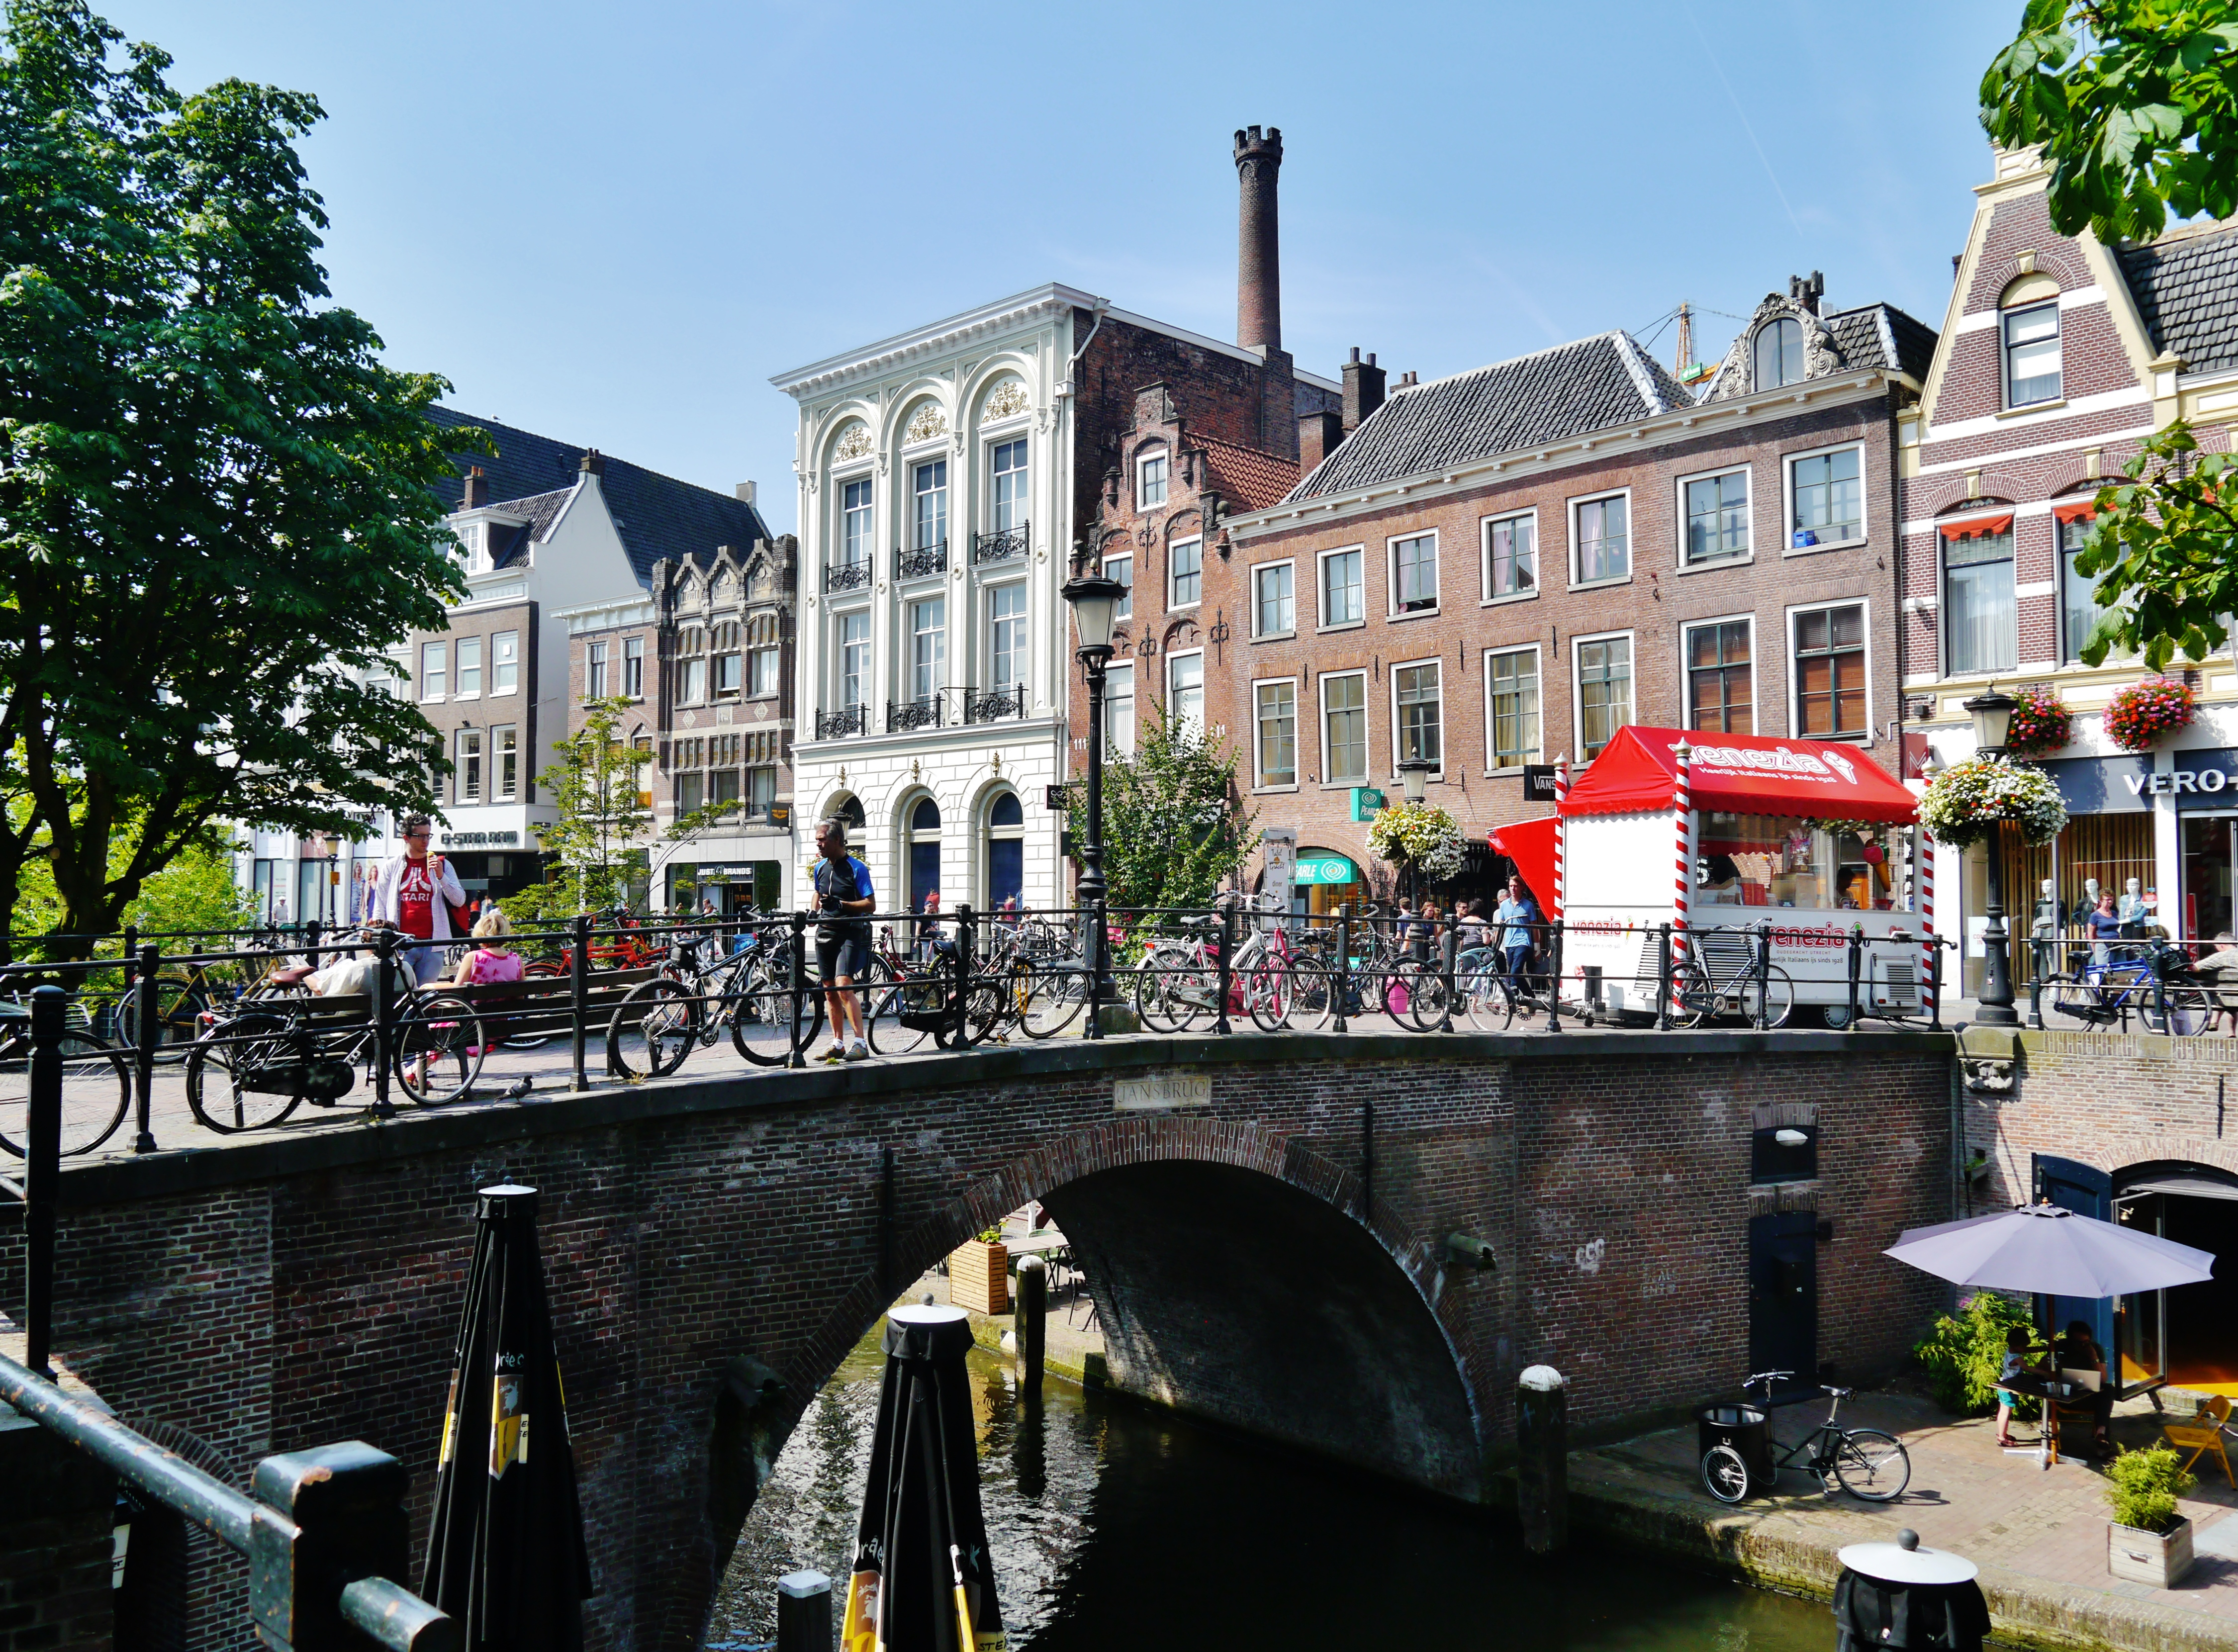
\includegraphics[width=0.7\linewidth]{images/utrecht1.jpg}
	\end{figure}
	\tiny\url{https://en.wikipedia.org/wiki/Utrecht}
	
\end{frame}

% get to destinations
% walkability
% some commutes enjoyable - break between activities


\begin{frame}

\textbf{Course Objectives}
		\small
		\begin{itemize}
			\item Understand fundamental concepts and theories in urban transportation geography and planning.
			
			\item Identify and critically assess major social, political, economic, and environmental issues related to urban transportation.
			
			\item Analyze and visualize transportation-related data (including using GIS) to describe travel behaviour, transportation networks, land use, and accessibility.
			
			\item Apply the theoretical and practical knowledge you have acquired from the course to develop recommendations on improving urban transport systems.
		\end{itemize}

\end{frame}





\begin{frame}
	\LARGE{\textbf{Course Outline}}
	
	\vspace{4mm}
	
	\small
	\textit{(open up the syllabus)}
\end{frame}

% TALK ABOUT A1!




\begin{frame}
	\LARGE{\textbf{Key Concepts in Urban Transportation}}
	\normalsize
	\vspace{4mm}
	\begin{itemize}
		\item Travel Demand
		\item Activity Participation
		\item Utility
		\item Travel Behaviour
		% \item Transport \& Land Use
		% \item Mobility VS Accessibility
	\end{itemize}
\end{frame}




\begin{frame}
	
	\textbf{Travel Demand}
	\vspace{4mm}
	
	\begin{itemize}
		\item Travel is often considered a \textit{derived demand} because we don’t directly benefit from it (usually)
		
		\item People travel because they want to consume a \textit{final good}
		
		\item The final good is \textbf{Activity Participation} (e.g., work, shopping, entertainment)
		 
		\item Travel is required to participate in activities that take place at different locations
	\end{itemize}
	
\end{frame}





\begin{frame}
	
	\textbf{Utility}
	\vspace{4mm}
	
	\begin{itemize}
		\item When trying to understand people’s travel decisions, we often assume that each individual is making the \textbf{best} choice for themselves
		
		\item \textbf{Utility} is a notion of how much benefit or satisfaction is derived from consuming a good
		
		\item Transportation planners/engineers assume that a travel choice is made to \textbf{maximize} one’s individual utility
	\end{itemize}
	
	
\end{frame}


\begin{frame}
	
	\textbf{Utility}
	\vspace{4mm}
	
	\begin{itemize}
		\item In the case of travel, it is generally assumed that travel is a	\textit{negative utility} (but not always!)
		
		\item \textit{Negative utility} is often framed in terms of \textbf{Costs} (e.g. monetary costs, time costs, stress, discomfort, etc.)
		
		\item People are therefore making choices that attempt to
		minimize the \textbf{disutility} of travel
		
		\item People take trips when the utility of travelling and activity participation are positive (i.e. outweigh the negatives)
	\end{itemize}
	
\end{frame}





\begin{frame}
	
	Example of \textit{positive utility} of travel:
	
	\vspace{3mm}
	
	\textit{The Ideal Commute Is Not Actually No Commute}
	
	- It's normal for people to want a little time to detach from the workplace.
	
	\begin{figure}
		\centering
		\includegraphics[width=0.7\linewidth]{images/commute_ideal.png}
	\end{figure}
	\tiny\url{https://www.bloomberg.com/news/articles/2014-08-06/the-ideal-commute-is-not-actually-no-commute}
	
	
\end{frame}





\begin{frame}
	
	\textbf{Travel Behaviour} - the study of how people travel
	
	\vspace{4mm}
	
	Trip Characteristics
	
	\begin{itemize}
		\item Where from?
		\item Where to?
		\item Why? (Activity Participation!)
		\item With Whom?
		\item When?
		\item How? (Mode Choice)
		\item Which route? (Route Selection)
	\end{itemize}
	
	
\end{frame}




\begin{frame}
	
	\textbf{Mode Choice} - i.e. which mode of travel should I use?
	\vspace{4mm}
	
	Pick the mode with the greatest utility (i.e. minimize dis-utility), based on the summation of various factors, e.g. consider two modes... 
	\vspace{2mm}
	
	\begin{figure}
		\centering
		\includegraphics[width=0.9\linewidth]{images/simple_mode_choice.png}
	\end{figure}

	What are some other factors?
	
	
\end{frame}





\begin{frame}
	
	\textbf{Route Selection} - i.e. which route should I take?
	\vspace{4mm}
	
	\begin{figure}
		\centering
		\includegraphics[width=0.98\linewidth]{images/bike_route_selection.png}
	\end{figure}
	
\end{frame}




\begin{frame}
	
	\textbf{Travel Behaviour} - the study of how people travel
	
	\vspace{4mm}
	
	Factors affecting travel behaviour are often divided into two categories
	
	\begin{enumerate}
		
		\item Urban spatial structure (locations of activities, transport networks)
		
		\item Individual attributes, preferences, and constraints
		
	\end{enumerate}


	\begin{figure}
		\centering
		\includegraphics[width=0.98\linewidth]{images/suburbs_tor.png}
	\end{figure}

\end{frame}




\begin{frame}
	
	Think about all the trips people take in a city ...
	
	\begin{figure}
		\centering
		\includegraphics[width=0.99\linewidth]{images/smto_stgeorge_all.png}
	\end{figure}
	\tiny\url{https://sausy-lab.github.io/SMTO_web_map/}
	
\end{frame}



\begin{frame}
	
	Big picture:
	
	\begin{figure}
	\centering
	\includegraphics[width=0.79\linewidth]{images/big_links.png}
	\end{figure}
	
\end{frame}




\begin{frame}
	
	\textbf{Transportation Demand Modelling}
	\vspace{4mm}
	
	\begin{itemize}
		
		\item Complex models built by transportation engineers to predict population-level distribution of trips in a region
		
		\item Use these predictions to help decide where new infrastructure should be built
		
		\item Often used as part of evaluating the costs and benefits between a set of alternatives (Cost-Benefit Analysis)
		
		\item Results have been used to justify new highways, transit lines, etc.
		
	\end{itemize}	
	
\end{frame}


\begin{frame}
	\textbf{Planning \& Design Challenges}
	\vspace{4mm}
	
	\begin{itemize}
		\item Lower GHG emissions
		\item Reduce congestion
		\item Safer streets
		\item Better accessibility
		\item Improving equity
		\item Affordability
		\item Encouraging active travel	
		\item etc.
		\item etc.
	\end{itemize}
	
\end{frame}



\begin{frame}
	
	\Large{\textbf{Activity!}}
	
	\vspace{4mm}
	
	\normalsize
	Which travel mode should be promoted most in the GTHA?
		
	\vspace{4mm}

	\begin{figure}
		\centering
		\includegraphics[width=0.3\linewidth]{images/mode_share_gtha_2016.png}
		\tiny{Source: 2016 Transportation Tomorrow Survey}
	\end{figure}

\end{frame}



	% Overview of what?
% system approach, 
% transport networks and land use
% social, env, econmoic impacts
% travel behaviour / trips

% concepts:

% utility
% demand
% mobility vs accessibility

% see SF slides 2

% transportationi is a complex system
% networks > land use > travel behaviour 

% networks slide

% land use slide

% trips slide

% what arer the qualities a trip?
% time, distance, mode, purpose
% subjective, satisfaction, etc.
% 




\begin{frame}
	\textbf{Next Week} 
	
	\vspace{4mm}
	
	Cars, Roads, \& Highways:
	
	\begin{itemize}
		
		% \item Mobility VS Accessibility
		
		\item Rise of cars as the predominant mode of travel in Canadian cities. 
		
		\item How the infrastructure of automobiles has transformed transportation and land-use and has affected daily life. 
	\end{itemize}

\end{frame}



\end{document}